% CVPR 2026 Paper Template; see https://github.com/cvpr-org/author-kit

\documentclass[10pt,twocolumn,letterpaper]{article}

%%%%%%%%% PAPER TYPE  - PLEASE UPDATE FOR FINAL VERSION
% \usepackage{cvpr}              % To produce the CAMERA-READY version
\usepackage{cvpr}      % To produce the REVIEW version
% \usepackage[pagenumbers]{cvpr} % To force page numbers, e.g. for an arXiv version

% Import additional packages in the preamble file, before hyperref
\input{preamble}

% It is strongly recommended to use hyperref, especially for the review version.
% hyperref with option pagebackref eases the reviewers' job.
% Please disable hyperref *only* if you encounter grave issues, 
% e.g. with the file validation for the camera-ready version.
%
% If you comment hyperref and then uncomment it, you should delete *.aux before re-running LaTeX.
% (Or just hit 'q' on the first LaTeX run, let it finish, and you should be clear).
\definecolor{cvprblue}{rgb}{0.21,0.49,0.74}
\usepackage[pagebackref,breaklinks,colorlinks,allcolors=cvprblue]{hyperref}

%%%%%%%%% PAPER ID  - PLEASE UPDATE
\def\paperID{*****} % *** Enter the Paper ID here
\def\confName{Meilenstein 3}
\def\confYear{2026}

\title{Abgabe \confName}

\author{Fabian Henßler
\and
Max Steidle
}

\begin{document}
\maketitle
\begin{abstract}
    Die automatisierte Klassifikation von Fernerkundungsbildern ist ein zentrales Problem in der Geoinformatik und bildet die Grundlage für Anwendungen wie Landnutzungskartierung, Stadtplanung und Umweltmonitoring.
    Aufbauend auf einer bereits untersuchten CNN-Baseline erweitert diese Arbeit den bisherigen Ansatz um Knowledge Distillation, um die Klassifikation von 38~PatternNet-Szenenklassen zu verbessern und zugleich ein kompakteres Modellverhalten zu untersuchen.
    Dazu wird zunächst ein leistungsfähiges Teacher-Modell auf dem PatternNet-Datensatz trainiert und anschließend ein kleineres Student-Modell mittels Distillation an dessen Vorhersagen angepasst.
    Die Modelle werden auf einer identischen Datenaufteilung unter vergleichbaren Trainingsbedingungen evaluiert und anhand von Validierungs- und Test-Accuracy sowie den Lernkurven miteinander verglichen.
    Die Ergebnisse zeigen, dass der Wissenstransfer vom Teacher zum Student die Leistung eines kleineren Netzes anheben kann, ohne die Modellkomplexität unnötig zu erhöhen.
    Insgesamt verdeutlicht die Arbeit, dass Knowledge Distillation einen sinnvollen Weg darstellt, um ein ausgewogenes Verhältnis zwischen Genauigkeit, Modellgröße und Trainingsaufwand zu erreichen.
\end{abstract}
\section{Einleitung}
\label{sec:einleitung}

% --- 1.1 Motivation ---
\subsection{Motivation und Problemstellung}
\label{subsec:motivation}

Die Klassifikation von Fernerkundungsbildern beschäftigt sich mit der Frage, welche Landnutzungs- oder Landbedeckungsklasse eine gegebene Bildszene repräsentiert.
Dies ist von hoher praktischer Relevanz, da Satelliten- und Luftbilder in immer größerem Umfang verfügbar werden und eine manuelle Auswertung dieser Datenmengen weder zeitlich noch wirtschaftlich realisierbar ist.
Automatisierte Verfahren sind daher unerlässlich, um beispielsweise Veränderungen in der Landnutzung zu erkennen, landwirtschaftliche Flächen zu überwachen oder Katastrophenschäden zu identifizieren.
Neben einer hohen Klassifikationsgenauigkeit spielen dabei auch Modellgröße, Inferenzzeit und Speicherbedarf eine wichtige Rolle, wenn Verfahren später effizient eingesetzt werden sollen.

% --- 1.2 Zielsetzung ---
\subsection{Zielsetzung der Arbeit}
\label{subsec:zielsetzung}

Ziel dieser Arbeit ist es, auf einer bereits vorhandenen CNN-Basis aufzubauen und zu untersuchen, wie sich Knowledge Distillation zur Verbesserung und Komprimierung des Modells einsetzen lässt.
Dazu wird ein leistungsfähiges Teacher-Modell als Referenz betrachtet und ein kleineres Student-Modell mithilfe von Distillation trainiert, sodass Wissen aus den Vorhersagen des Teachers auf das kompaktere Netz übertragen wird.
Im Vordergrund steht damit nicht mehr der reine Architekturvergleich, sondern die Frage, ob sich mit Distillation ein gutes Verhältnis zwischen Klassifikationsleistung und Modellkomplexität erreichen lässt.

Im Rahmen dieser Arbeit werden insbesondere folgende Fragen betrachtet:
\begin{itemize}
	\item Wie stark kann ein Student-Modell durch Knowledge Distillation gegenüber einem ohne Distillation trainierten Modell profitieren?
	\item Welche Auswirkungen hat der Wissenstransfer auf Trainingsverlauf, Validierungsverhalten und Test-Accuracy?
	\item Lässt sich die Modellgröße reduzieren, ohne die Klassifikationsleistung unverhältnismäßig zu verschlechtern?
\end{itemize}

% --- 1.3 Aufbau der Arbeit ---
\subsection{Aufbau der Arbeit}
\label{subsec:aufbau}

Der weitere Bericht ist wie folgt gegliedert:
Nach dieser Einleitung folgt in Abschnitt~\ref{sec:stand-der-forschung} der Stand der Forschung zu CNN-basierten Verfahren und Knowledge Distillation.
Abschnitt~\ref{sec:methode} beschreibt den Datensatz, die Vorverarbeitung, die Netzarchitektur, das Knowledge-Distillation-Verfahren sowie Trainings- und Implementierungsdetails.
In Abschnitt~\ref{sec:ergebnisse} werden das experimentelle Setup, die quantitativen Resultate und die klassenweise Analyse anhand der Konfusionsmatrizen präsentiert.
Abschnitt~\ref{sec:diskussion} ordnet die Ergebnisse in den Kontext der vorangegangenen Meilensteine ein und diskutiert insbesondere den Einfluss der Hyperparameter.
Abschnitt~\ref{sec:fazit} fasst die wesentlichen Erkenntnisse der Arbeit zusammen.
Abschließend folgt ein kurzer Abschnitt zur Verfügbarkeit von Code und Datensatz, bevor im Anhang ergänzende Materialien folgen.
\section{Stand der Forschung}
\label{sec:stand-der-forschung}

In der ersten Arbeit \cite{steidlehenssler2026milestone1} wurde eine Reihe von CNN-Architekturen für die Klassifikation von Szenen aus dem PatternNet-Datensatz untersucht.
Dabei standen vor allem der systematische Vergleich verschiedener Modellvarianten sowie der Einfluss von Architekturelementen wie Batch-Normalisierung, Dropout, Pooling und der Tiefe des Netzes im Mittelpunkt.
Die Ergebnisse dieser Vorarbeit lieferten eine belastbare CNN-Basis und zeigten, dass insbesondere batch-normalisierte Architekturen die beste Klassifikationsleistung erzielen.

Die vorliegende Arbeit baut auf dieser Grundlage auf und erweitert den bisherigen Ansatz um Knowledge Distillation.
Anstelle eines reinen Architekturvergleichs wird nun ein Teacher-Student-Setup betrachtet, in dem ein leistungsfähigeres Teacher-Modell Wissen an ein kompakteres Student-Modell überträgt.
Zusätzlich zur klassischen Auswertung der Test-Accuracy wird damit auch untersucht, wie sich der Wissenstransfer auf das Lernverhalten und das Leistungsniveau eines kleineren Modells auswirkt.

Im Vergleich zur ersten Arbeit liegt der zusätzliche Beitrag somit in der Distillation-Komponente selbst: Das Student-Modell soll nicht nur aus den harten Labels lernen, sondern auch von den weicheren Vorhersagen des Teachers profitieren.
Damit verschiebt sich der Fokus von der Frage, welche CNN-Architektur allein am besten abschneidet, hin zu der Frage, wie sich eine bereits gute Modellbasis durch Knowledge Distillation weiter verbessern und effizienter machen lässt.
\section{Eigene Methoden}
\label{sec:methode}

\subsection{Datensatz}
\label{subsec:datensatz}

Grundlage der Experimente ist derselbe PatternNet-Datensatz wie in der ersten Arbeit~\cite{steidlehenssler2026milestone1}.
Für die hier untersuchten Distillation-Experimente wurde die Stichprobe wie zuvor auf 100 Bilder pro Klasse begrenzt, damit die Ergebnisse direkt vergleichbar bleiben.

\subsection{Vorverarbeitung und Datenaugmentation}
\label{subsec:augmentation}

Die genaue Vorverarbeitung, Datenaugmentation, Normalisierung und Aufteilung des Datensatzes entsprechen der ersten Arbeit~\cite{steidlehenssler2026milestone1} und werden hier nicht erneut im Detail wiederholt.
Für die vorliegenden Distillation-Experimente wurden diese Schritte unverändert übernommen, um die Vergleichbarkeit mit der Vorarbeit zu sichern.

\subsection{Netzarchitektur}
\label{subsec:architektur}

Die Knowledge-Distillation-Experimente bestehen aus zwei Netzen: einem Teacher und einem Student.
Als Teacher wurde das beste Modell aus den Transfer-Learning-Experimenten verwendet, ein ResNet50 mit dem besten dort erzielten Ergebnis von etwa 97\,\%.
Als Student dient ein abgeschwächtes Modell auf Basis des Base\_Net aus der ersten Arbeit~\cite{steidlehenssler2026milestone1}, das zusätzlich um Batch-Normalisierung erweitert wurde.
Damit bleibt der Student deutlich kleiner als der Teacher, erhält aber eine stabilere Trainingsdynamik als das ursprüngliche Basismodell.

Beide Netze geben vor der Softmax-Aktivierung Logits aus.
Diese Logits sind die Grundlage für die Distillation, da nicht nur die harten Klassenlabels, sondern auch die weichen Vorhersagen des Teachers in die Optimierung einfließen.
Das grundlegende Prinzip der Knowledge Distillation folgt dabei der Arbeit von Hinton et al.~\cite{hinton2015distilling}.

\subsection{Knowledge Distillation}
\label{subsec:distillation}

Seien $z_s$ die Logits des Student-Modells und $z_t$ die Logits des Teacher-Modells.
Aus diesen Werten werden temperaturgeskalierte Verteilungen berechnet:
\begin{equation}
  p_s^{(T)} = \operatorname{softmax}\left(\frac{z_s}{T}\right),
  \qquad
  p_t^{(T)} = \operatorname{softmax}\left(\frac{z_t}{T}\right).
\end{equation}
Die Temperatur $T$ steuert die Weichheit der Verteilungen. Höhere Temperaturen glätten die Wahrscheinlichkeiten und machen Nebenklassen sichtbarer, während kleinere Temperaturen die Verteilungen schärfer machen.

Die verwendete Distillation-Loss kombiniert den Kreuzentropie-Term mit einer KL-Divergenz zwischen Teacher- und Student-Verteilungen:
\begin{equation}
  \mathcal{L}_{\mathrm{KD}} = \alpha \, \mathcal{L}_{\mathrm{CE}}(y, z_s)
  + (1-\alpha) \, T^2 \, \mathcal{L}_{\mathrm{KL}}\left(p_t^{(T)}, p_s^{(T)}\right).
\end{equation}
Dabei ist $y$ das Ground-Truth-Label, $\mathcal{L}_{\mathrm{CE}}$ der Kreuzentropie-Term und $\mathcal{L}_{\mathrm{KL}}$ die Kullback-Leibler-Divergenz zwischen den temperaturgeskalierten Verteilungen.
Der Faktor $T^2$ kompensiert dabei den Skalierungseffekt der Temperatur auf die Gradienten und hält den Beitrag des Distillation-Terms in einem vergleichbaren numerischen Bereich.
Der Parameter $\alpha$ gewichtet das Verhältnis zwischen den harten Labels und dem Wissen des Teachers.

\subsection{Trainingsverfahren}
\label{subsec:training}

Alle Läufe wurden unter identischen Bedingungen trainiert, um die verschiedenen Distillationseinstellungen direkt vergleichen zu können.
Als Optimizer wurde Adam mit den Standardparametern der PyTorch-Implementierung verwendet ($\eta = 10^{-3}$; $\beta_1 = 0{,}9$; $\beta_2 = 0{,}999$).
Ein Learning-Rate-Scheduler wurde nicht eingesetzt, sodass die Lernrate über alle Epochen konstant blieb.

Das Training erfolgte über 15~Epochen mit einer Batchgröße von 64.
Für die Distillation wurden die Temperaturen $T \in \{2; 4; 6\}$ und die $\alpha$-Werte $\alpha \in \{{,}1; {,}2; {,}3\}$ untersucht.
Damit ergaben sich insgesamt neun Durchläufe, in denen jede Temperatur mit jedem Alpha-Wert kombiniert wurde.

Die Bewertung erfolgte primär über die Test-Accuracy.
Zusätzlich wurden nach jeder Epoche die Validierungs-Accuracy und der Validierungs-Loss berechnet und mit TensorBoard protokolliert.
Auch die Konfusionsmatrix wurde auf der Validierungsmenge pro Epoche erstellt, um klassenspezifische Fehlklassifikationen sichtbar zu machen.

\subsection{Implementierungsdetails}
\label{subsec:implementierung}

Die technischen Details zur Dataset-Klasse, zur Stratifizierung, zur DataLoader-Konfiguration sowie zum Logging entsprechen ebenfalls weitgehend der ersten Arbeit~\cite{steidlehenssler2026milestone1}.
Für die hier untersuchten Distillation-Läufe wurden diese Bestandteile nicht neu konzipiert, sondern als gemeinsame Infrastruktur übernommen, damit der Effekt von Teacher, Student sowie Temperatur und $\alpha$ isoliert untersucht werden kann.

\subsection{Evaluationsmetrik}
\label{subsec:evaluation}

Zur Bewertung der Klassifikationsleistung wird die \textit{Accuracy} (Genauigkeit) herangezogen, definiert als der Anteil korrekt klassifizierter Bilder an der Gesamtzahl der Testbilder:
\begin{equation}
  \text{Accuracy} = \frac{\text{Anzahl korrekt klassifizierter Bilder}}{\text{Gesamtzahl der Testbilder}}
\end{equation}

Da der PatternNet-Datensatz gleichverteilte Klassen aufweist, ist die Accuracy eine aussagekräftige Metrik, die nicht durch Klassenungleichgewichte verzerrt wird.
Darüber hinaus wurde die Konfusionsmatrix verwendet, um die Verteilung der Fehlklassifikationen über die Klassen hinweg zu analysieren und potenzielle Schwächen des Modells in Bezug auf bestimmte Klassen zu identifizieren.
\section{Ergebnisse}
\label{sec:ergebnisse}

\subsection{Experimentelles Setup}
In diesem Kapitel werden die Ergebnisse der in Kapitel~\ref{sec:methode} beschriebenen 
Experimente vorgestellt und analysiert. Untersucht wurde, inwiefern sich die Klassifikationsleistung
eines kompakten Student-Netzes durch Knowledge Distillation von einem größeren Teacher-Modell verbessern 
lässt. Als Vergleichsbasis dient das identische Student-Netz, das ohne Teacher ausschließlich mit den 
Ground-Truth-Labels trainiert wurde. Die Bewertung erfolgt anhand der Test- und Validierungsgenauigkeit, 
der Verlustverläufe während des Trainings sowie einer klassenweisen Analyse mittels Konfusionsmatrizen.

\subsection{Quantitative Ergebnisse}
\label{sec:quantitative_ergebnisse}
 
Tabelle~\ref{tab:distillation_ergebnisse} fasst die Ergebnisse aller Trainingsläufe zusammen. Insgesamt
liegen die erzielten Testgenauigkeiten in einem Bereich von 71{,}40\,\% bis 82{,}11\,\% und damit auf einem
grundsätzlich vergleichbaren Niveau. Innerhalb dieses Bereichs zeigen sich jedoch deutliche Unterschiede in
Abhängigkeit von der Wahl der Hyperparameter $\alpha$ (Gewichtung zwischen Distillations- und Klassifikationsverlust)
und $T$ (Temperatur der Softmax-Funktion).
 
Besonders hervorzuheben ist die Konfiguration $\alpha = 0{,}1$ und $T = 4{,}0$: Mit einer Testgenauigkeit von
82{,}11\,\% erzielt sie das mit Abstand beste Ergebnis aller Versuche. Gegenüber der Baseline von 73{,}16\,\% entspricht
dies einer absoluten Verbesserung von rund 9~Prozentpunkten bzw. einer relativen Steigerung von etwa 12\,\%. Dieses
Modell erreicht zudem mit 84{,}04\,\% die höchste Validierungsgenauigkeit und mit 0{,}671 den niedrigsten
Validierungsverlust aller Läufe, was auf eine konsistent bessere Generalisierung und nicht lediglich auf einen zufälligen
Ausreißer hindeutet.
 
Die beobachtete Verbesserung stellt sich jedoch nicht in allen Konfigurationen ein. Zwei Kombinationen --
$\alpha = 0{,}1$, $T = 2{,}0$ (71{,}40\,\%) sowie $\alpha = 0{,}3$, $T = 2{,}0$ (72{,}98\,\%) -- schneiden sogar
schlechter ab als die Baseline. Auffällig ist, dass beide unterlegenen Läufe mit der niedrigsten untersuchten
Temperatur $T = 2{,}0$ trainiert wurden, mit Ausnahme der Konfiguration $\alpha = 0{,}2$, $T = 2{,}0$, die mit
78{,}95\,\% überdurchschnittlich abschneidet. Weitere Konfigurationen, etwa $\alpha = 0{,}3$ mit $T = 6{,}0$
(74{,}39\,\%), liegen nur unwesentlich über der Baseline und weisen damit keine praktisch relevante Verbesserung auf.
Ein streng monotoner Zusammenhang zwischen den Hyperparametern und der erzielten Genauigkeit lässt sich aus den Daten
nicht ableiten; vielmehr deutet sich an, dass eine geringe Gewichtung des Hard-Label-Verlusts ($\alpha = 0{,}1$) in
Kombination mit einer moderaten Temperatur ($T = 4{,}0$) das Wissen des Teachers am effektivsten überträgt.
 
Hinsichtlich des Rechenaufwands ist festzuhalten, dass die Distillation die Trainingszeit von etwa 2{,}4~Minuten
auf 6{,}6 bis 7{,}7~Minuten nahezu verdreifacht, da in jedem Trainingsschritt zusätzlich ein Forward-Pass durch das
Teacher-Modell erforderlich ist. Da dieser Mehraufwand ausschließlich das Training betrifft und die Inferenzkosten des
Student-Netzes unverändert bleiben, ist er für den angestrebten Einsatzzweck eines kompakten Modells unkritisch.
 
Anzumerken ist außerdem, dass die absoluten Werte des Trainingsverlusts der destillierten Modelle
(vgl. Abbildungen~\ref{fig:train_loss} und \ref{fig:val_loss}) nicht direkt mit dem der Baseline vergleichbar sind, da sich die Verlustfunktion
der Distillation aus der gewichteten Summe von Kreuzentropie- und Kullback-Leibler-Term zusammensetzt und Letzterer
mit $T^2$ skaliert. Die durchweg höheren Trainingsverluste bei größeren Temperaturen sind daher konstruktionsbedingt
und kein Indiz für schlechtere Konvergenz. Die Validierungsverluste, die für alle Modelle einheitlich als Kreuzentropie
berechnet werden, bestätigen hingegen die Rangfolge der Genauigkeiten.
 
\subsection{Konfusionsmatrix und klassenweise Analyse}
 
Für eine differenziertere Betrachtung werden die Konfusionsmatrizen des besten destillierten Modells 
($\alpha = 0{,}1$, $T = 4{,}0$, Abbildung~\ref{fig:cm_distilled}) und der Baseline (Abbildung~\ref{fig:cm_baseline}) 
gegenübergestellt. Grundsätzlich weisen die Matrizen aller Läufe ein ähnliches Muster auf: Die Stärken und Schwächen 
konzentrieren sich auf dieselben Klassen und unterscheiden sich zwischen den Konfigurationen meist nur in Details.
 
Visuell eindeutig unterscheidbare Klassen wie \textit{beach}, \textit{cemetery}, \textit{chaparral}, \textit{freeway},
\textit{oil\_gas\_field}, \textit{oil\_well}, \textit{parking\_lot} und \textit{solar\_panel} werden von beiden Modellen
nahezu fehlerfrei klassifiziert. Die systematischen Verwechslungen treten hingegen erwartungsgemäß zwischen semantisch
und visuell verwandten Klassen auf. Hierzu zählen insbesondere:
 
\begin{itemize}
	\item \textit{sparse\_residential} und \textit{dense\_residential}, die sich primär in der Bebauungsdichte unterscheiden,
	\item \textit{basketball\_court} und \textit{tennis\_court}, die als rechteckige Sportflächen eine sehr ähnliche Struktur aufweisen,
	\item \textit{runway} und \textit{runway\_marking}, die denselben Bildinhalt in unterschiedlichem Maßstab zeigen,
	\item Klassen mit Wasser- bzw. Hafenbezug wie \textit{ferry\_terminal}, \textit{harbor} und \textit{bridge}.
\end{itemize}
 
Der Vergleich der beiden Matrizen zeigt, dass die Distillation vor allem bei diesen schwierigen Klassen zu Verbesserungen
führt. Besonders deutlich wird dies bei \textit{dense\_residential}: Während die Baseline hier lediglich 6 von 15
Testbildern korrekt zuordnet und die übrigen überwiegend auf benachbarte Bebauungsklassen verteilt, klassifiziert das
destillierte Modell alle 15 Bilder korrekt. Ähnliche Zugewinne zeigen sich bei \textit{nursing\_home}
(10 statt 6 korrekte Zuordnungen), \textit{parking\_space} (13 statt 6) und \textit{crosswalk} (15 statt 11). Diese
Beobachtung stützt die Hypothese, dass die weichen Wahrscheinlichkeitsverteilungen des Teachers gerade bei ähnlichen
Klassen zusätzliche Information über deren Beziehungen zueinander liefern, die aus den harten Labels allein nicht
hervorgeht.
 
Vereinzelt verschlechtert sich die Erkennung einzelner Klassen durch die Distillation geringfügig, etwa bei
\textit{storage\_tank} (11 statt 12 korrekte Zuordnungen) oder \textit{airplain}. In der Gesamtbilanz überwiegen 
die Verbesserungen jedoch klar, was sich in der um rund 9~Prozentpunkte höheren Gesamtgenauigkeit widerspiegelt.
 
\subsection{Interpretation und qualitative Beobachtungen}
 
Zusammenfassend lässt sich festhalten, dass die Wahl der Hyperparameter $\alpha$ und $T$ das Ergebnis der Knowledge
Distillation maßgeblich beeinflusst. Nicht jede Kombination führt zu der erhofften Verbesserung: Zwei der neun
untersuchten Konfigurationen blieben hinter der Baseline zurück, weitere erreichten lediglich ein vergleichbares Niveau.
In der Mehrzahl der Fälle bewirkte die Distillation jedoch eine Steigerung der Testgenauigkeit in der Größenordnung von
3 bis 5~Prozentpunkten; in der besten Konfiguration ($\alpha = 0{,}1$, $T = 4{,}0$) betrug der Zugewinn sogar
rund 9~Prozentpunkte.
 
Die Ergebnisse legen nahe, dass eine niedrige Gewichtung des Hard-Label-Anteils in Verbindung mit einer moderaten
Temperatur am besten geeignet ist, das im Teacher enthaltene Wissen über die Ähnlichkeitsstruktur der Klassen auf das
Student-Netz zu übertragen. Bei zu niedriger Temperatur nähern sich die weichen Zielverteilungen den harten Labels an,
sodass der zusätzliche Informationsgehalt weitgehend verloren geht; dies bietet eine plausible Erklärung für das schwache
Abschneiden mehrerer Läufe mit $T = 2{,}0$. Die klassenweise Analyse bestätigt darüber hinaus, dass der Nutzen der
Distillation vor allem bei visuell schwer unterscheidbaren Klassen zum Tragen kommt, während bei ohnehin gut separierbaren
Klassen kaum Spielraum für Verbesserungen besteht.

\section{Diskussion}
\label{sec:diskussion}
 
In diesem Abschnitt werden die Ergebnisse der Knowledge Distillation in den Kontext der beiden vorangegangenen
Meilensteine eingeordnet, die auf demselben Datensatz durchgeführt wurden. In Meilenstein~1 wurden zehn selbst
entworfene CNN-Architekturen von Grund auf trainiert, in Meilenstein~2 wurden vortrainierte ResNet-Modelle
(ResNet-18 bis ResNet-152) mittels Transfer Learning angepasst. Das beste Modell aus Meilenstein~2 diente anschließend
als Teacher für die in dieser Arbeit untersuchte Distillation. Abschließend werden die bereits in
Abschnitt~\ref{sec:quantitative_ergebnisse} beobachteten Effekte der Hyperparameter $\alpha$ und $T$ vertiefend
analysiert.
 
\subsection{Vergleich mit den Architekturen aus Meilenstein~1}
\label{sec:diskussion_m1}
 
Besonders aufschlussreich ist der Vergleich mit Meilenstein~1, da die dort untersuchten Architekturen hinsichtlich der
Parameteranzahl in einer ähnlichen Größenordnung liegen wie das Student-Netz, jedoch durchweg tiefer sind, also über mehr
Schichten verfügen (vgl. Tabelle~\ref{tab:architektur_uebersicht}). Der Vergleich erlaubt daher eine Einschätzung,
inwieweit Knowledge Distillation den Nachteil einer geringeren Netztiefe kompensieren kann.
 
Als direkteste Vergleichsgruppe eignen sich die Architekturen mit Batch-Normalisierung, da auch das Student-Netz diese
Technik einsetzt. Das ohne Teacher trainierte Student-Netz erreicht mit einer Testgenauigkeit von 73{,}16\,\% ein
Ergebnis, das unterhalb aller BatchNorm-Varianten aus Meilenstein~1 liegt: Bereits das einfache \textit{BatchNorm\_Net}
erzielt 79{,}6\,\%, die beste Architektur \textit{BatchNorm\_Dense\_Pool\_Conv\_Net} sogar 84{,}2\,\%. Lediglich
das \textit{BatchNorm\_Dense\_Pool\_Net} liegt mit 73{,}0\,\% auf demselben Niveau wie die Baseline. Dieser Rückstand
ist plausibel auf die geringere Tiefe des Student-Netzes zurückzuführen, die dessen Repräsentationsfähigkeit einschränkt.
 
Durch die Knowledge Distillation verschiebt sich dieses Bild deutlich: Das beste destillierte Modell
($\alpha = 0{,}1$, $T = 4{,}0$) erreicht mit 82{,}11\,\% eine Testgenauigkeit, die nur noch rund 2~Prozentpunkte
unter der besten Architektur aus Meilenstein~1 liegt und drei der fünf BatchNorm-Varianten übertrifft. Das flachere
Student-Netz kommt mit Unterstützung des Teachers also nahezu an das Ergebnis heran, für das in Meilenstein~1 eine
tiefere und aufwendig per Architektursuche optimierte Netzstruktur erforderlich war. Dies deutet darauf hin, dass ein
wesentlicher Teil des Leistungsunterschieds zwischen flachen und tiefen Netzen dieser Größenordnung nicht in der
Kapazität der Netze selbst begründet liegt, sondern in der Qualität des Trainingssignals: Die weichen Zielverteilungen
des Teachers stellen dem Student-Netz zusätzliche Information über die Ähnlichkeitsstruktur der Klassen bereit, die aus
den harten Labels allein nicht hervorgeht.
 
\subsection{Vergleich mit den Transfer-Learning-Modellen aus Meilenstein~2}
\label{sec:diskussion_m2}
 
Die mittels Transfer Learning angepassten ResNet-Modelle aus Meilenstein~2 markieren die obere Leistungsgrenze in dieser
Versuchsreihe: Alle fünf Varianten erreichen Validierungsgenauigkeiten zwischen 96{,}8\,\% und 98{,}9\,\%, wobei das
ResNet-50 mit 98{,}95\,\% am besten abschneidet und daher als Teacher für die Distillation ausgewählt wurde. Auffällig
ist, dass die Leistung innerhalb der ResNet-Familie kaum mit der Netztiefe skaliert was darauf hindeutet, dass die auf ImageNet
vorgelernten Merkmale für den vorliegenden Datensatz bereits weitgehend ausreichen und die Aufgabe für diese Modellklasse nicht
kapazitätslimitiert ist.
 
Gegenüber dem Teacher verbleibt auch nach der Distillation eine erhebliche Lücke von rund 15~Prozentpunkten
(82{,}11\,\% gegenüber 98{,}95\,\%). Das Student-Netz kann das Wissen des Teachers also nur teilweise übernehmen,
was angesichts des großen Kapazitäts- und Tiefenunterschieds sowie des fehlenden Vortrainings zu erwarten war. Die
Distillation ist somit kein Ersatz für Transfer Learning, wenn maximale Genauigkeit das Ziel ist. Sie schließt jedoch
einen relevanten Teil der Lücke zwischen dem frei trainierten Student-Netz und dem Teacher: Von den ursprünglich rund
26~Prozentpunkten Abstand zwischen Baseline und Teacher werden etwa 9~Prozentpunkte durch die Distillation
zurückgewonnen. Für Einsatzszenarien mit beschränkten Ressourcen, etwa auf eingebetteten Systemen, stellt der destillierte Student
daher einen attraktiven Kompromiss zwischen Genauigkeit und Modellgröße dar.
 
\subsection{Einfluss der Hyperparameter}
\label{sec:diskussion_hyperparameter}
 
Die in Abschnitt~\ref{sec:quantitative_ergebnisse} dargestellten Ergebnisse zeigen, dass der Erfolg der Distillation
empfindlich von der Wahl der Hyperparameter $\alpha$ und $T$ abhängt. Über die Konfigurationen hinweg schwankt die
Testgenauigkeit um mehr als 10~Prozentpunkte (71{,}40\,\% bis 82{,}11\,\%), und zwei Kombinationen bleiben sogar
hinter der Baseline ohne Teacher zurück. Eine ungünstige Parameterwahl kann den Nutzen der Distillation demnach nicht
nur aufheben, sondern das Training aktiv verschlechtern.
 
Bei der Temperatur deutet sich ein systematischer Effekt an: Zwei der drei Läufe mit $T = 2{,}0$ zählen zu den
schwächsten Ergebnissen. Eine niedrige Temperatur lässt die weichen Zielverteilungen des Teachers gegen die harten
Labels konvergieren, wodurch der zusätzliche Informationsgehalt über die Klassenähnlichkeiten weitgehend verloren
geht -- der Student erhält dann im Wesentlichen ein redundantes, aber verrauschtes zweites Label-Signal. Die moderate
Temperatur $T = 4{,}0$ erweist sich in Kombination mit $\alpha = 0{,}1$ als optimal, während $T = 6{,}0$ die
Verteilungen bereits so stark glättet, dass die Ergebnisse wieder leicht abfallen.
 
Beim Gewichtungsfaktor zeigt sich, dass die beste Leistung bei der kleinsten untersuchten Gewichtung des
Hard-Label-Anteils ($\alpha = 0{,}1$) erzielt wird, das Signal des Teachers also stark dominieren sollte. Dies ist
konsistent mit der hohen Qualität des Teachers: Bei einer Genauigkeit von annähernd 99\,\% sind dessen Vorhersagen
fast immer korrekt und zugleich informativer als die harten Labels, sodass eine stärkere Gewichtung der
Ground-Truth-Labels kaum zusätzlichen Nutzen stiftet. Ein streng monotoner Zusammenhang lässt sich allerdings weder
für $\alpha$ noch für $T$ ableiten; die Wechselwirkung beider Parameter ist offensichtlich nichtlinear. Da jede
Konfiguration nur zweimal trainiert wurde, ist zudem nicht auszuschließen, dass ein Teil der beobachteten Unterschiede
auf die Zufallsinitialisierung zurückgeht.

\section{Zusammenfassung}
\label{sec:fazit}

Über die drei Meilensteine hinweg ergibt sich ein konsistentes Gesamtbild: Transfer Learning mit vortrainierten
ResNets liefert auf dem untersuchten Datensatz die mit Abstand höchste Genauigkeit ($\approx 99\,\%$), erfordert
jedoch große Modelle. Selbst entworfene tiefe CNNs erreichen nach sorgfältiger Architektursuche bis zu 84{,}2\,\%.
Knowledge Distillation ermöglicht es einem bewusst kompakten und flachen Student-Netz, mit 82{,}11\,\% nahezu zu
diesen aufwendig optimierten Architekturen aufzuschließen und seine eigene Baseline um rund 9~Prozentpunkte zu
übertreffen. Dies erfordert jedoch eine sorgfältige Hyperparameterwahl. Die Methode ist damit insbesondere dann
attraktiv, wenn ein starker Teacher bereits vorhanden ist und die Modellgröße durch die Zielplattform beschränkt wird.

\input{sec/7_availability}
% Bibliographie vor dem Anhang platzieren
{
    \small
    \bibliographystyle{ieeenat_fullname}
    \bibliography{main}
}

\appendix
\clearpage
\onecolumn
 
\setcounter{page}{1}
\maketitlesupplementary
 
\section{Ergänzende Abbildungen}
\label{sec:supp_figures}
 
% ----------------------------------------------------------
% Seite 1: beide Tabellen in natürlicher Größe
% ----------------------------------------------------------
 
\begin{table}[H]
	\centering
	\caption{Vergleich der Trainingsläufe: Testgenauigkeit, Validierungsgenauigkeit und Validierungsverlust nach 15 Epochen sowie die benötigte Trainingszeit. Als Baseline dient das ohne Teacher trainierte Student-Netz. Das beste Ergebnis ist fett hervorgehoben.}
	\label{tab:distillation_ergebnisse}
	\begin{tabular}{llrrrr}
		\toprule
		$\alpha$ & $T$ & Acc\textsubscript{Test} [\%] & Acc\textsubscript{Val} [\%] & Loss\textsubscript{Val} & Zeit [min] \\
		\midrule
		\multicolumn{2}{l}{Baseline (ohne Teacher)} & 73{,}16 & 75{,}44 & 0{,}899 & 2{,}44 \\
		\midrule
		0{,}1 & 2{,}0 & 71{,}40          & 72{,}28          & 1{,}492          & 6{,}57 \\
		0{,}1 & 4{,}0 & \textbf{82{,}11} & \textbf{84{,}04} & \textbf{0{,}671} & 6{,}65 \\
		0{,}1 & 6{,}0 & 77{,}37          & 79{,}65          & 1{,}058          & 6{,}66 \\
		0{,}2 & 2{,}0 & 78{,}95          & 79{,}12          & 0{,}870          & 6{,}70 \\
		0{,}2 & 4{,}0 & 76{,}49          & 75{,}96          & 1{,}370          & 6{,}75 \\
		0{,}2 & 6{,}0 & 80{,}18          & 77{,}72          & 1{,}038          & 6{,}75 \\
		0{,}3 & 2{,}0 & 72{,}98          & 75{,}61          & 1{,}093          & 7{,}68 \\
		0{,}3 & 4{,}0 & 76{,}84          & 79{,}47          & 0{,}971          & 6{,}71 \\
		0{,}3 & 6{,}0 & 74{,}39          & 74{,}91          & 1{,}301          & 6{,}84 \\
		\bottomrule
	\end{tabular}
\end{table}
 
\vspace{1.5em}
 
\begin{table}[H]
	\centering
	\caption{Übersicht der getesteten Netzarchitekturen. Conv = Anzahl Convolution-Layern, Pool = Anzahl Max-Pooling-Schichten, FC = Anzahl vollständig verbundener Schichten (inkl. Ausgabeschicht), BN = Batch-Normalisierung, DO = Dropout ($p = 0{,}5$).}
	\label{tab:architektur_uebersicht}
	\begin{tabular}{llccccc}
		\toprule
		\textbf{Phase} & \textbf{Netzwerk}                              & \textbf{Conv} & \textbf{Pool} & \textbf{FC} & \textbf{BN} & \textbf{DO} \\
		\midrule
		1              & Base\_Net                                      & 5             & 2 + GAP       & 3           & --          & --          \\
		\midrule
		2              & Conv\_Net                                      & 8             & 2             & 3           & --          & --          \\
		2              & Dense\_Net                                     & 5             & 2             & 7           & --          & --          \\
		2              & Pooling\_Net                                   & 5             & 4             & 3           & --          & --          \\
		2              & Dropout\_Net                                   & 5             & 2             & 3           & --          & \checkmark  \\
		2              & BatchNorm\_Net                                 & 5             & 2             & 3           & \checkmark  & --          \\
		\midrule
		3              & BatchNorm\_Dense\_Pool\_Net                    & 5             & 3             & 4           & \checkmark  & --          \\
		3              & BatchNorm\_Dense\_Pool\_Conv\_Net              & 6             & 3             & 4           & \checkmark  & --          \\
		3              & BatchNorm\_Dense\_Pool\_Conv\_Dropout\_Net     & 6             & 3             & 4           & \checkmark  & \checkmark  \\
		3              & BatchNorm\_Dense\_Pool\_Conv\_Dropout\_V2\_Net & 6             & 3             & 4           & \checkmark  & \checkmark  \\
		\bottomrule
	\end{tabular}
\end{table}
 
\clearpage
\onecolumn
% ----------------------------------------------------------
% Seite 2: Loss-Verläufe
% ----------------------------------------------------------
 
\begin{figure}[H]
	\centering
	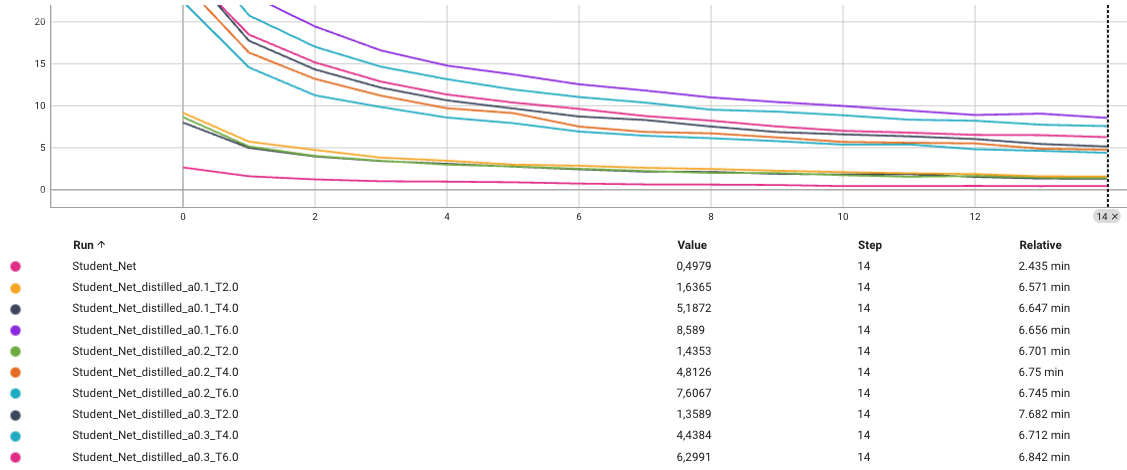
\includegraphics[width=\linewidth, height=0.85\textheight, keepaspectratio]{figures/loss.png}
	\caption{Verlauf des Trainingsverlusts über 15 Epochen für alle Konfigurationen.}
	\label{fig:train_loss}
\end{figure}

\begin{figure}[H]
	\centering
	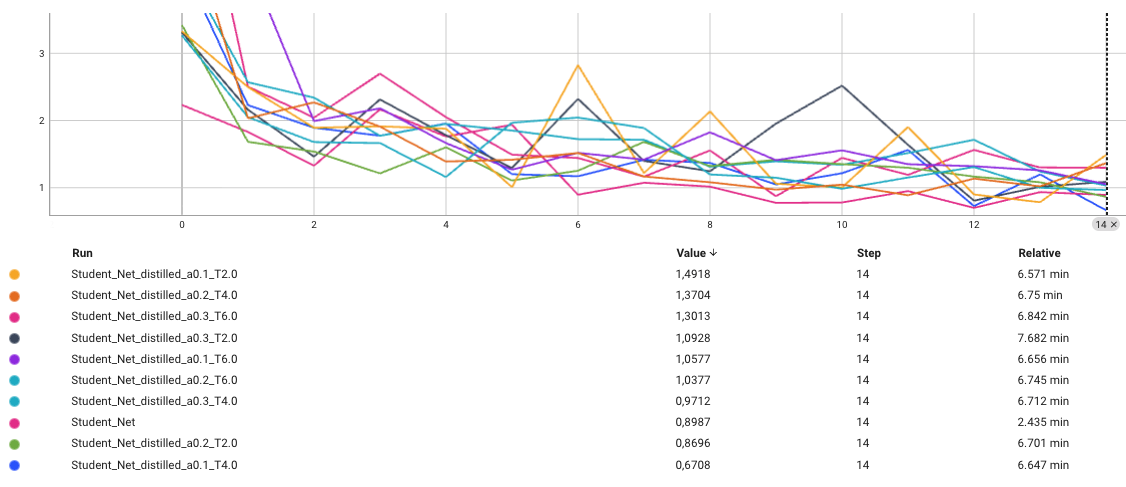
\includegraphics[width=\linewidth, height=0.85\textheight, keepaspectratio]{figures/val_loss.png}
	\caption{Verlauf des Validierungsverlusts über 15 Epochen für alle Konfigurationen.}
	\label{fig:val_loss}
\end{figure}
 
\clearpage
\onecolumn

% ----------------------------------------------------------
% Seite 3 und 4: je eine Konfusionsmatrix pro Seite
% ----------------------------------------------------------
 
\begin{figure}[H]
	\centering
	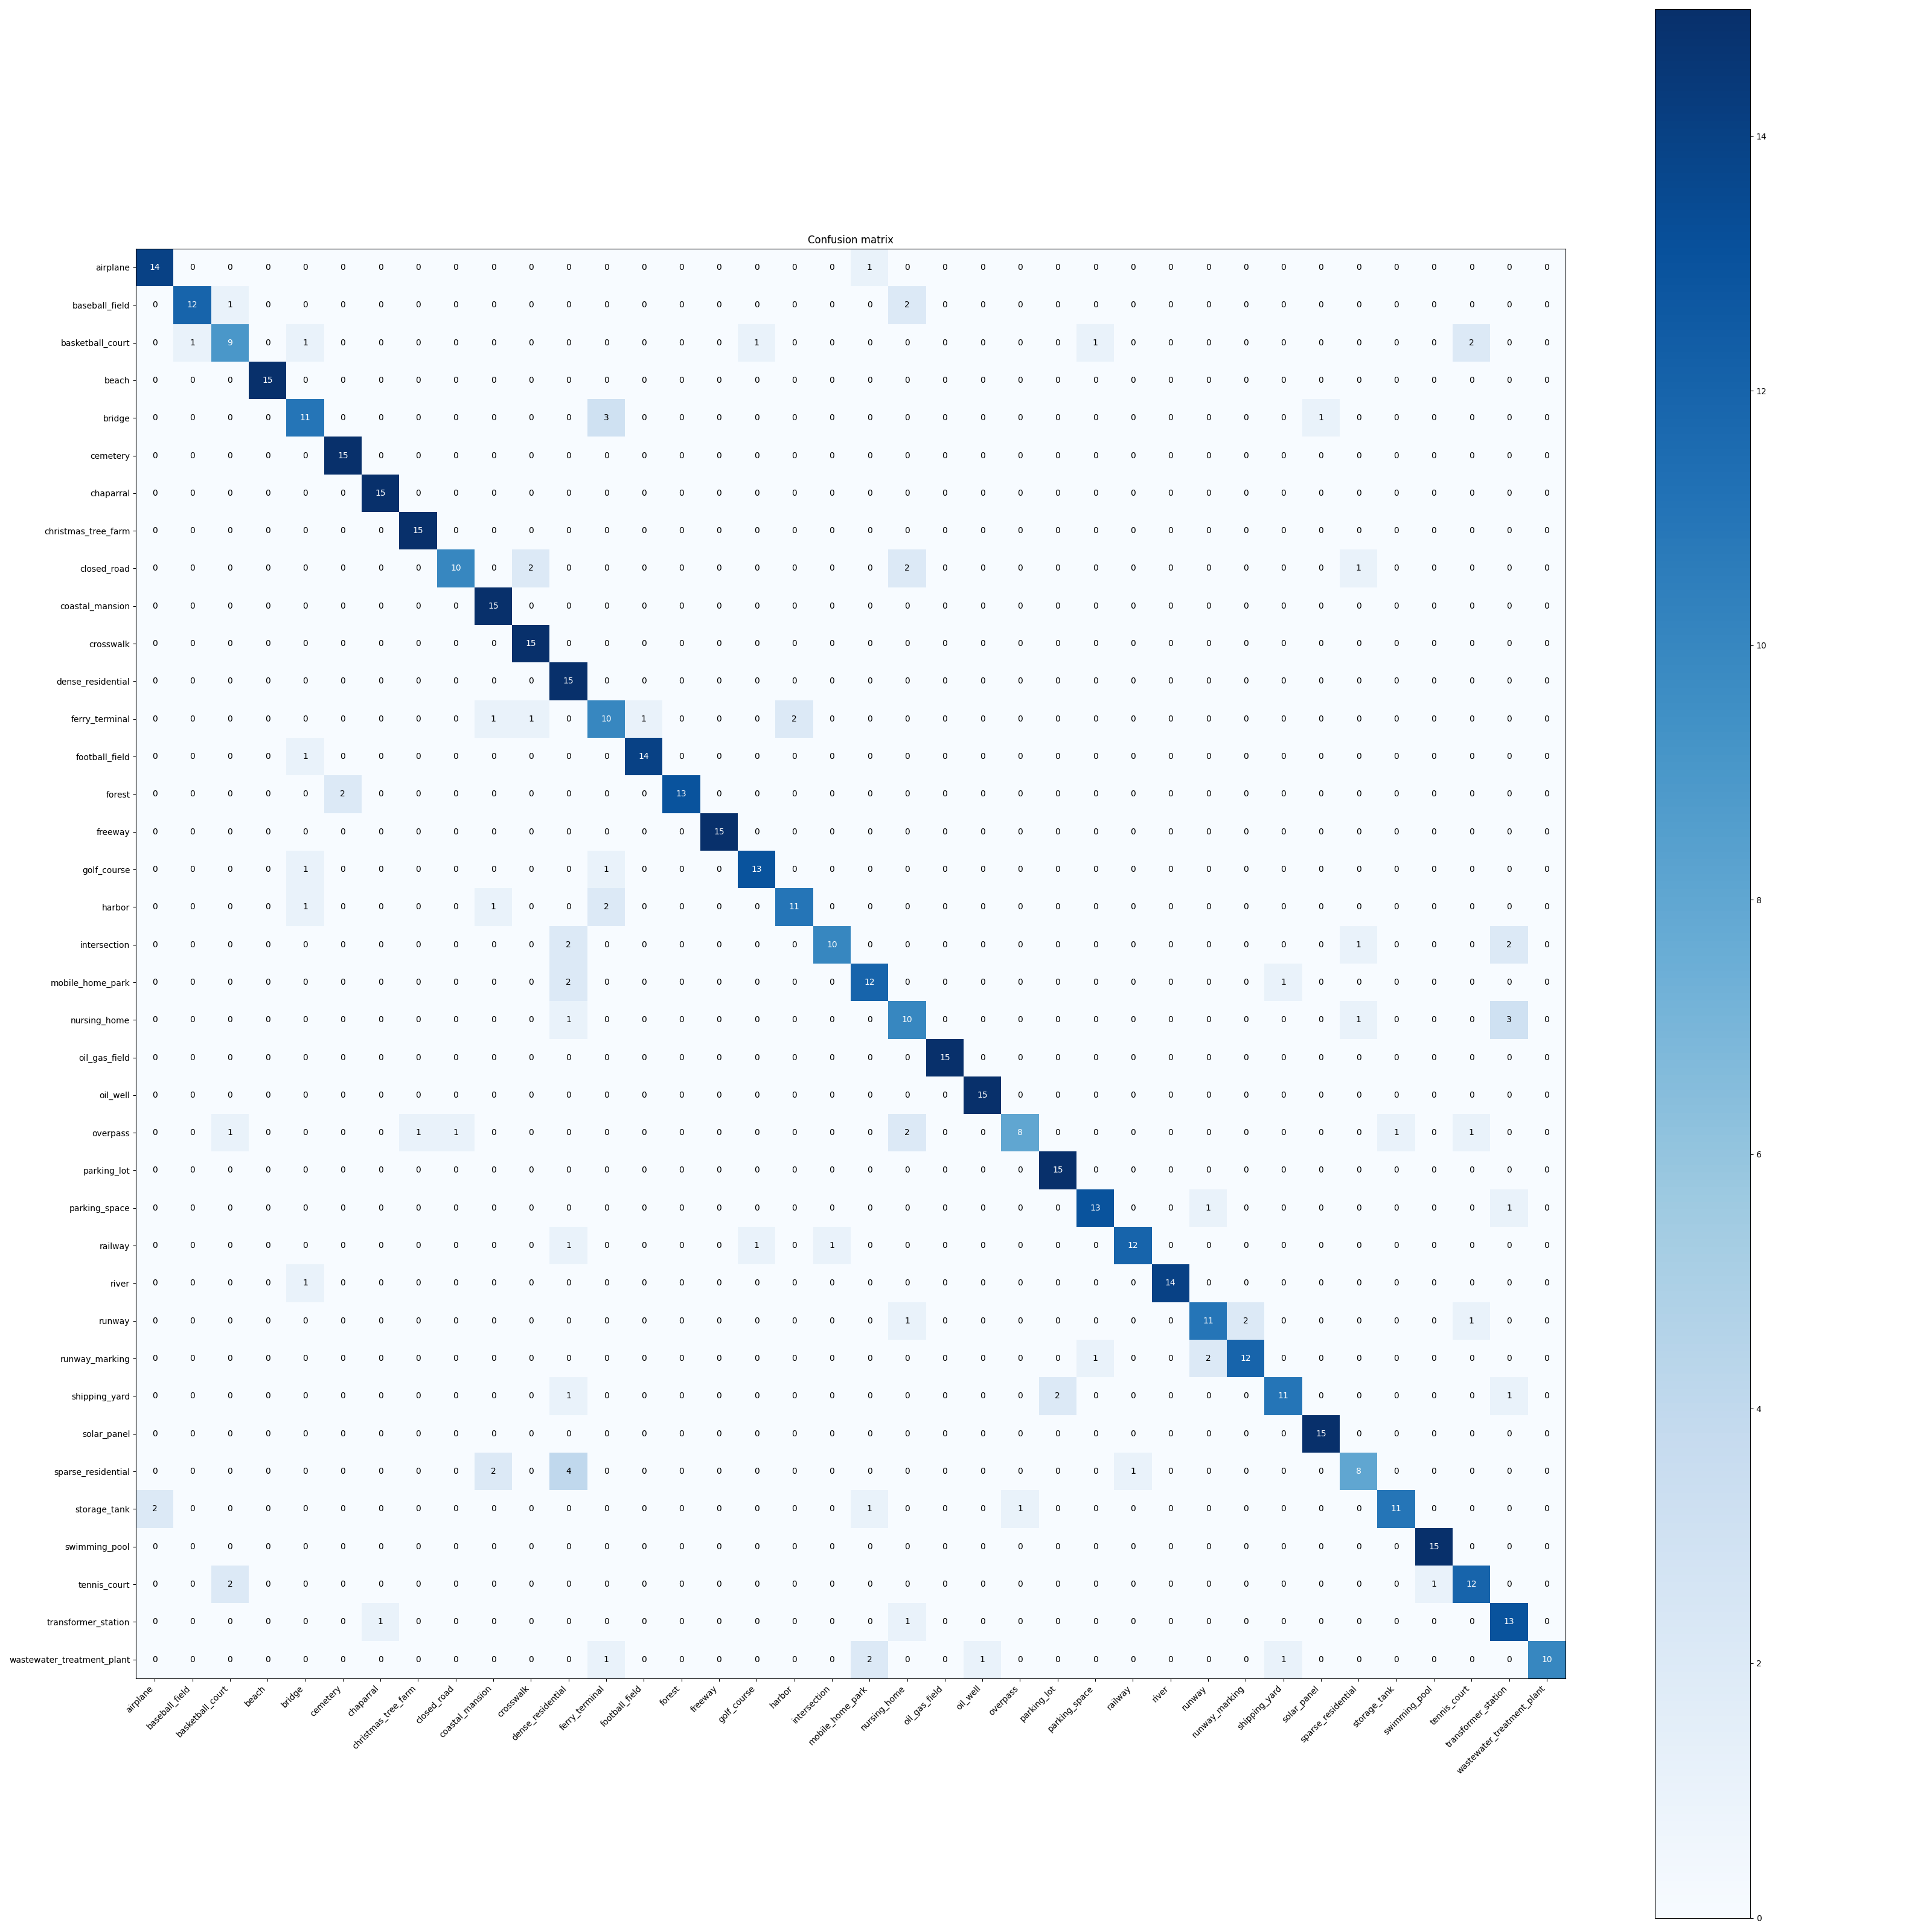
\includegraphics[width=\linewidth, height=0.88\textheight, keepaspectratio]{figures/cm_distilled_a01_T4.png}
	\caption{Konfusionsmatrix des besten destillierten Modells ($\alpha = 0{,}1$, $T = 4{,}0$) auf dem Testdatensatz.}
	\label{fig:cm_distilled}
\end{figure}
 
\clearpage
 
\begin{figure}[H]
	\centering
	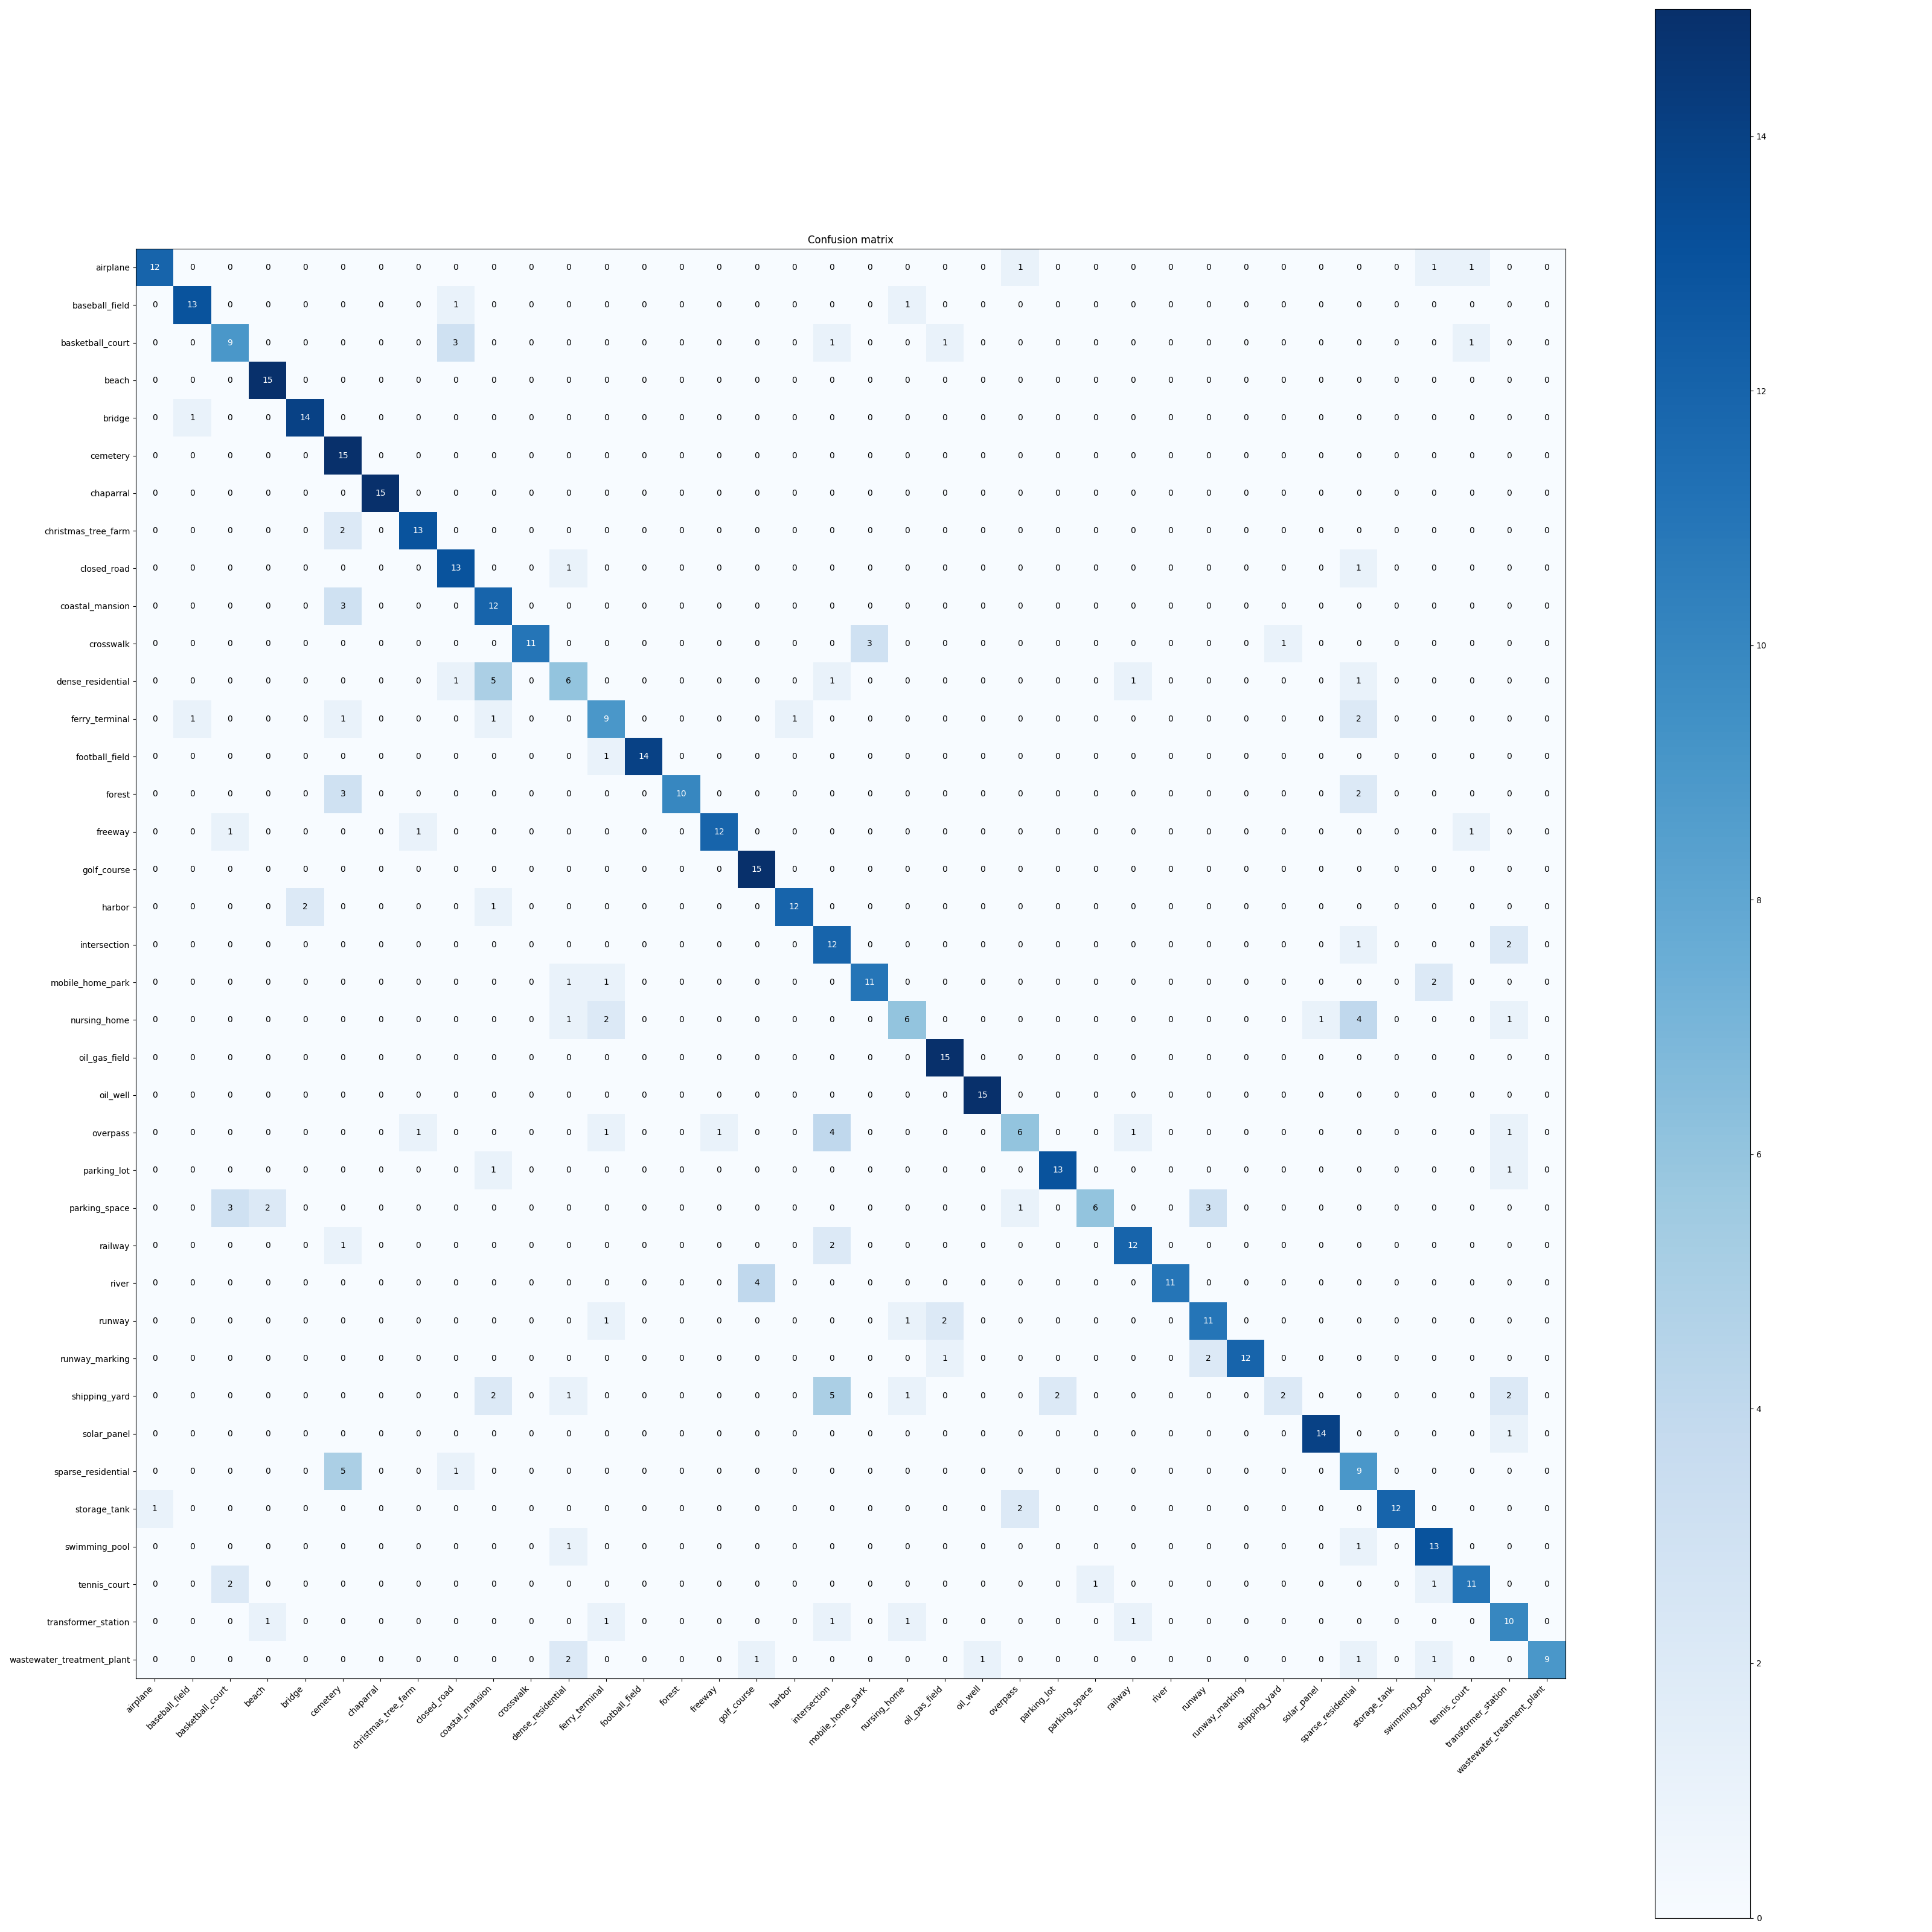
\includegraphics[width=\linewidth, height=0.88\textheight, keepaspectratio]{figures/cm_baseline.png}
	\caption{Konfusionsmatrix des ohne Teacher trainierten Student-Netzes (Baseline) auf dem Testdatensatz.}
	\label{fig:cm_baseline}
\end{figure}

% WARNING: do not forget to delete the supplementary pages from your submission 

\end{document}
